% DOCUMENT FORMATTING

\documentclass[10.5pt,a4paper]{article} % Document type and paper size

\usepackage[margin={1cm,1cm}]{geometry} % Margins 
\usepackage{multicol} % For the two column layout
\usepackage{graphicx} % For includegraphics / images command
\usepackage{color} % Colour of fonts
\usepackage[dvipsnames]{xcolor} % Colour of text boxes 
\usepackage{parskip}  % For gaps between paragraphs 
\usepackage[hidelinks]{hyperref} % For clickable hyperlinks (the "hidelinks" part hides the light blue box around hyperlinks)
\usepackage{titlesec} % Needed to set section and subsection header spacing below
\usepackage[T1]{fontenc} % Font used for main body + titles

\setlength{\columnsep}{1cm} % Centeral gap between columns
\graphicspath{ {images/} } % Graphics location
\renewcommand*\rmdefault{pag} % Set font
\pagenumbering{gobble} % Disables page numbering

\titlespacing\section{0pt}{12pt plus 4pt minus 2pt}{0pt plus 2pt minus 2pt}
\titlespacing\subsection{0pt}{12pt plus 4pt minus 2pt}{0pt plus 2pt minus 2pt}
\titlespacing\subsubsection{0pt}{12pt plus 4pt minus 2pt}{0pt plus 2pt minus 2pt} 
% Spacing between different content types



% DOCUMENT CONTENT

\begin{document} % Document content below this point

\begin{center}
	\vspace{1cm}
	\colorbox{Black}{
		\begin{minipage}{18.5cm}
			\begin{center}
			\color{white}
			\vspace{0.3cm}
	             
\includegraphics[width=1\textwidth]{organisationlogo.eps} % Organisation Logo
	        \\[10pt]
			     \textbf{{\LARGE CRYPTOPARTYNEWCASTLE.ORG}} % WEB URL
			\vspace{0.3cm}
			\end{center}
		\end{minipage}
	}
\end{center}
% Document Header


\begin{center}
\vspace{0.5cm}
\textbf{{\LARGE Using the Tor Browser on Windows} % Leaflet Header
\vspace{0.5cm}
}\end{center}
% Document Title


\begin{multicols*}{2} % Two Column Layout

The Tor Browser is a customised version of the free-and-open-source Firefox web browser that makes it easy to protect your browsing activity by passing it through the Tor network.


\section*{Installation}
To install the Tor Browser on Windows, navigate to the link below. Do not use any other source, and do not proceed if you receive a certificate error.

\begin{center}
	\url{https://www.torproject.org/download/} % Clickable URL.
\end{center}

Expand the `Microsoft Windows' section, and click the `Download Tor Browser' button:
\begin{center}
	
\includegraphics[width=0.25\textwidth]{downloadbutton.png} % Embed image from the images folder
\end{center}

Save the downloaded file somewhere, and then open it to install the Tor Browser. You will be asked to choose a location for the browser to be installed into. Your user folder is probably a good choice.


\section*{First Launch}
When you first launch the Tor Browser, you will see a prompt (below) asking you whether you wish to connect directly to the Tor network.

\begin{center}
	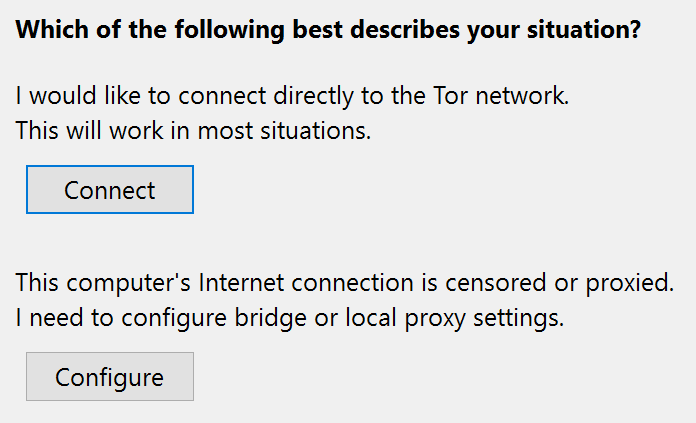
\includegraphics[width=0.40\textwidth]{first-run.png}
\end{center}

If you are connecting to Tor from a country with heavily censored internet access, please seek additional information and advice before choosing to directly connect to Tor at the above prompt.

However, in most cases, UK users will want to select the option to connect directly to the Tor network.


\section*{Settings}
The Tor Browser features a security panel (which you can open from the Onion icon on your browser toolbar). This `Onion Menu' has a slider allowing you to adjust the browser's security level.

\begin{center}
	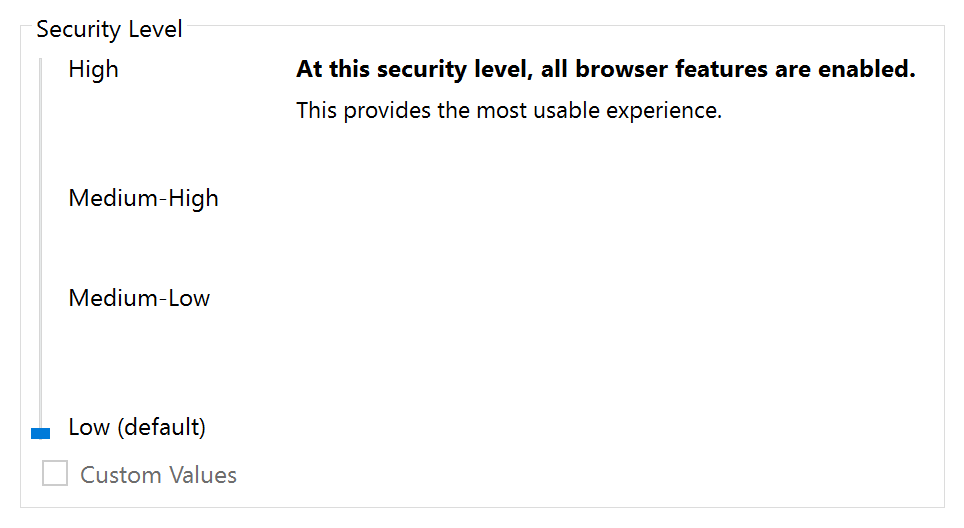
\includegraphics[width=0.30\textwidth]{onion-menu.png}
\end{center}

Some features of a normal web browser may reveal your identity to a site, or make you vulnerable to attacks. Turning the security slider to a high setting disables some of these features, making you safer from well-funded attackers who can interfere with your internet connection, or use new unknown vulnerabilities in these features.

Unfortunately, turning off some of these features can lead to some websites that use them becoming unusable. The default `Low' setting is fine for everday privacy protecion, but you can choose to set it to `High' if you are worried about sophisticated attackers, or if you don't mind that some websites may display incorrectly.


\section*{Browser Add-ons}
For security purposes, the Tor Project team recommend you do not install additional Add-ons into the Tor Browser, as they may interfere with how Tor works and cause the browser to leak your identity to the sites you visit.


\section*{Usage}
That's it! You can now use the Tor Browser as you would use a normal web browser, and browse the internet while protecting your privacy and anonymity.

You may wish to read the Tor Project website for more detailed information on staying secure.


\begin{center}
	\vfill % Blank vertical space until box starts in bottom corner.
	\colorbox{Black}{
		\begin{minipage}{8cm}
			\color{white}
			\vspace{0.2cm}
			\begin{center}
				\textbf{{\Large Please visit \url{torproject.org}\\for more information.}}
			\end{center}
			\vspace{0.2cm}
		\end{minipage}
	}
\end{center}

\vspace{0.75cm}

\end{multicols*}

\end{document}
